% Chapter Template

\chapter{Cell segmentation} % Main chapter title

\label{Chapter4} % Change X to a consecutive number; for referencing this chapter elsewhere, use \ref{ChapterX}


%----------------------------------------------------------------------------------------
%	INTRODUCTION
%----------------------------------------------------------------------------------------

Finding the cells in images is the first and crucial step in the procedure. The problems encountered in cell segmentation are discussed in Chapter \ref{Chapter3}. All of the problems occur due to colouring procedure that is time dependent, so cells expose different properties over an image and some of them remain undetected. Second problem that occur is that a part of the cells overlap. The challenge here is to find a method that can overcome different illumination of objects and separate the overlapping objects. The proposed solution deals with mentioned problems in separate steps. \\


The proposed solution is based on an observation that, although cells exhibit different properties across image due to different illumination levels, the background is uniform over a whole image and exhibits constant properties. Following the observations, the method first segments the background to find locations of the cells and then uses the second segmentation step to refine the borders of cells. \\



%----------------------------------------%
%                                        %
%         REGION GROWING                 %
%                                        %
%----------------------------------------%


\section{Background segmentation}

The first step of background segmentation is intended to overcome the problem of undetected cells. A desirable property of the segmentation approach for this task is the capability of capturing global properties of the background region across an image. One such algorithm is \textit{Region growing}. Region growing is a simple method that extends a region based on a similarity in intensity levels - the intensity of each candidate pixel is compared with a mean intensity of a current region. If a difference is less than a given threshold, the pixel is added to region. \\

The algorithm is summarized in algorithm \ref{alg:RegGrow}. It starts with a single point, adds its neighbours to the candidate region and compares their intensity to the mean intensity of the region. If a candidate point satisfies the criteria, it is added to the region and its neighbours become candidate points. The process is repeated while there are candidate points to be tested. \\

\begin{algorithm}
\caption{Region Growing }
  \label{alg:RegGrow}
\begin{algorithmic}[1]
 \Function{RegionGrowing}{\textit{starting point, criteria}}
 \State $\mathtt{candidates} \gets \{ \mathtt{neighborhood}(\mathtt{starting \ point}) \}$
 \State $\mathtt{region} \gets \{ \mathtt{starting \ point} \}$
 \State $\mathtt{current point} \gets \mathtt{starting \ point}$
 \While{new candidates}
 	\For{each candidate of current point}
 		\If{candidate satisfies criteria}
 			\State add it to region
 			\State update parameters of region
 		\EndIf 
 	\EndFor
 	\State $\mathtt{current point} \gets \mathtt{next \ point \ from \ border}$
 \EndWhile
 \EndFunction
\end{algorithmic}
\end{algorithm}

The bottleneck of the method is the evaluation of candidate pixels. If target regions are big, as in this case, the method could be very slow. To overcome this bottle neck, the method is extended with a pre-filling step in which a part of an image is assigned to belong to the background by default. As it can be noticed from the images, the majority of the image is a dark background which can be observed in an image histogram as the highest peak. To speed up the segmentation, every pixel with an intensity lower or equal to the highest peak is automatically assigned to the  background.   \\

The issue here is the estimation of a threshold for comparison. It is a parameter that depends on a distribution of intensities over an image. In a sense, this parameter models a variance in intensity of the background region. Motivated by variance fitting, the proposed solution is based on an assumption that an image histogram should consist of two regions - one modelling the background and a second one modelling cells, as illustrated in image \ref{img:Histogram}. The goal now is to find those two regions in the histogram. One way to accomplish that is to approximate the histogram with a mixture of Gaussian functions. This approach is taken here.  

\begin{figure}
	\begin{center}
		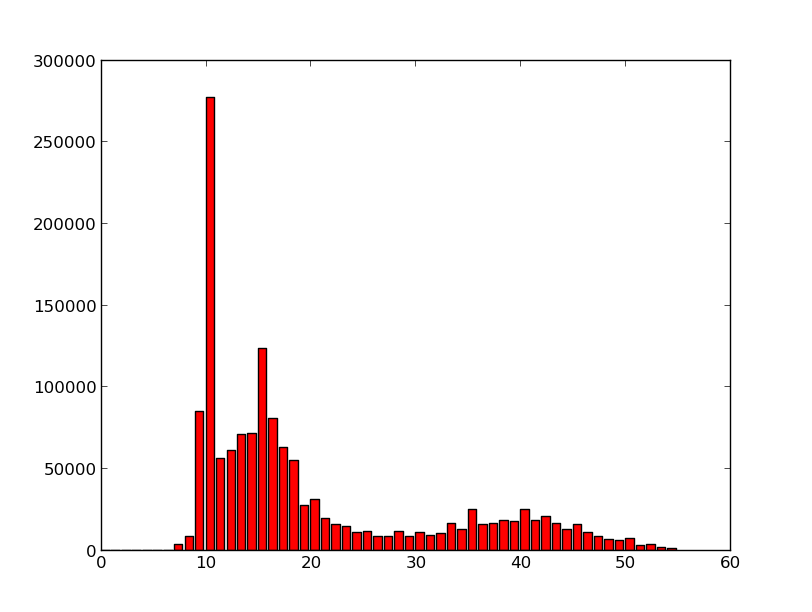
\includegraphics[scale=0.4]{Figures/segmentation/raw_histogram}
		\caption{Example of an image histogram}
		\label{img:Histogram}
	\end{center}
\end{figure}

%-----------------------------------------------------------------------------------------
%     GAUSSIAN MIXTURE MODELS
%-----------------------------------------------------------------------------------------

\subsection{Gaussian mixture model} 

Mixture density is a linear combination of \textit{K} probabilistic density functions:

\begin{equation}
	p(\mathbf{x}) = \sum_{k=1}^{K}\pi_k p(\mathbf{x} | \boldsymbol \theta_k)
	\label{eq:GMM}
\end{equation}
	 
where $p(\mathbf{x} | \theta_k)$ represents mixture components with their parameters $\theta_k$. In this case, these mixture components are Gaussian functions $\mathcal{N}(\mu_k, \Sigma_k)$. Parameters $\pi_k$ are mixture coefficients that satisfy $0 \leq \pi_k \leq 1$ and $\sum_{k=1}^{K} \pi_k = 1$. As they satisfy the given criteria, these coefficients can be treated as prior probability of a component $k$. Equation \ref{eq:GMM} can be then rewritten as :

\begin{equation}
	p(\mathbf{x}) = \sum_{k=1}^{K} P(\mathcal{G}_k) p(\mathbf{x} | \mathcal{G}_k),
\end{equation}

where $P(\mathcal{G}) = \pi_k$ and $ p(\mathbf{x} | \boldsymbol \theta_k) =  p(\mathbf{x} | \mathcal{G}_k)$. The task now is to determine the parameters

\begin{equation}
	 \boldsymbol \theta = \{ P(\mathcal{G}_k),  \theta_k \}_{k=1}^K,
\end{equation}


or more precisely for the Gaussian function

\begin{equation}
	 \boldsymbol \theta = \{ P(\mathcal{G}_k), \mu_k, \Sigma_k \}_{k=1}^K.
\end{equation}


An efficient algorithm to determine those values is the Expectation Maximization algorithm.



%------------------------------------------------------------------------------------------
%     EM ALGORITHM
%------------------------------------------------------------------------------------------

\subsection{Expectation Maximization Algorithm}

The goal of the Expectation Maximization algorithm is to find parameters $\boldsymbol \theta$ that maximize the log-likelihood 

\begin{equation}
	\mathcal{L}(\theta | \mathcal{D}) = \mathtt{ln}\prod_{i=1}^{N}p(\mathbf{x}^{(i)}) = \mathtt{ln}\prod_{i=1}^{N}\sum_{k=1}^{K}p(\mathbf{x}^{(i)} | \theta_k) = \sum_{i=1}^{N}\mathtt{ln}\sum_{k=1}^{K}p(\mathbf{x}^{(i)} | \theta_k).
\end{equation}

Unfortunately, there is no closed-form solution for this formulation. Model $p( \mathbf{X} | \boldsymbol \theta)$ is extended with latent variable $\mathbf{Z}$ which determines to which cluster  every $x_i$ belongs. The density function is now described with $p(\mathbf{X}, \mathbf{Z} | \boldsymbol \theta)$. Marginal density $p(\mathbf{X} | \theta)$, which is the density of interest, can always be reconstructed from a joint probability by marginalization :

$$ p(\mathbf{X} | \theta) = \sum_{\mathbf{Z}}p(\mathbf{X}, \mathbf{Z} | \boldsymbol \theta). $$

The log-likelihood that has to be maximized is now 

\begin{equation}
	\mathtt{ln}\mathcal{L}(\boldsymbol \theta | \mathbf{X}) = \mathtt{ln}p(\mathbf{X} | \boldsymbol \theta) = \mathtt{ln}\sum_{\mathbf{Z}}p(\mathbf{X}, \mathbf{Z} | \boldsymbol \theta).
\end{equation}

As values of the latent variable $\mathbf{Z}$ are not yet known, the log-likelihood cannot still be used directly. Instead,  the expectation of the log-likelihood $\mathbb{E}[ \mathtt{ln} \mathcal{L}(\boldsymbol \theta | \mathbf{X}, \mathbf{Z}) ]$ is used. The main idea behind the EM-algorithm is to iteratively adjust parameters $\boldsymbol \theta$ to maximize the expectation. \\

The maximization of  $\mathbb{E}[ \mathtt{ln} \mathcal{L}(\boldsymbol \theta | \mathbf{X}, \mathbf{Z}) ]$ is now done by switching between two steps -- E-step and M-step. E-step (\textit{expectation step}) calculates the expectation of the log-likelihood with respect to the current values of the parameters  $ \boldsymbol\theta^{(t)}$. That expectation $\mathcal{Q}( \boldsymbol \theta | \boldsymbol \theta^{(t)})$ can be calculated as

\begin{equation} \label{eq1}
\begin{split}
  \mathcal{Q}(\boldsymbol \theta | \boldsymbol \theta^{(t)}) &= \mathbb{E}_{\mathbf{Z} | \mathbf{X}, \boldsymbol \theta^{(t)}}[ \mathtt{ln} \mathcal{L}(\theta | \mathbf{X}, \mathbf{Z}) ] \\
     &= \mathbb{E}_{\mathbf{Z} | \mathbf{X}, \theta^{(t)}}[ \mathtt{ln} p(\mathbf{X}, \mathbf{Z} | \theta) ] \\
      &= \sum_{\mathbf{Z}}P(\mathbf{Z}| \mathbf{X}, \boldsymbol \theta^{(t)})\mathtt{ln} p(\mathbf{X}, \mathbf{Z} | \boldsymbol \theta). \\
\end{split}
\end{equation}

The expectation is now expressed on variable $\mathbf{Z}$ with fixed values of $\mathbf{X}$ and $\boldsymbol \theta$. Probability $P(\mathbf{Z}| \mathbf{X}, \boldsymbol \theta^{(t)})$ is the \textit{a posteriori } probability of the latent variable $\mathbf{Z}$ with fixed parameters which can be evaluated using Bayes rule. \\

The only thing left is to optimize the parameters $\boldsymbol \theta$. M-step (\textit{maximization step}) chooses new parameters $\boldsymbol \theta^{(t+1)}$ by maximizing the expression

\begin{equation}
	\boldsymbol \theta^{(t+1)} = \arg \max_{\theta}\mathcal{Q}(\boldsymbol \theta | \boldsymbol \theta^{(t)}).
\end{equation}
The EM-algorithm is briefly summarized in Algorithm \ref{alg:EM}. Starting with the initial parameters $\boldsymbol \theta^{(0)}$, it iteratively switches between E and M step until converged. The convergence is guaranteed as the algorithm maximizes the expectation in every iteration. On the other hand, the found solution might not be the global optimum. \\

\begin{algorithm}
\label{alg:EM}
\caption{Expectation-maximization algorithm}

\begin{algorithmic}[1]
 	\Function{EM}{}
 		\State Initialize parameters $\boldsymbol \theta^{(0)}$
 		\State \textit{t} $\leftarrow$ 0
 		\Repeat
 			\State \textbf{E-step:} calculate $P(\mathbf{Z} | \mathbf{X}, \boldsymbol \theta^{(t)})$
 			\State \textbf{M-step:} $\boldsymbol \theta^{(t+1)} \leftarrow \arg\max_{\theta}\mathcal{Q}(\boldsymbol \theta | \boldsymbol \theta^{(t)})$ 
 			 \Statex \quad \quad \quad \quad where $\mathcal{Q}(\boldsymbol \theta | \boldsymbol \theta^{(t)}) = \sum_{\mathbf{Z}}P(\mathbf{Z}|\mathbf{X}, \boldsymbol \theta^{(t)}) \mathtt{ln}p(\mathbf{X}, \mathbf{Z}| \boldsymbol \theta)$
 			\State $t \leftarrow t+1$
 		\Until{converged}
 	\EndFunction
\end{algorithmic}
\end{algorithm}


%---------------------------------------------%
%                                             %
%               EM for GMM                    %
%                                             %
%---------------------------------------------%



\subsection{EM algorithm for mixture models}

The EM-algorithm for mixture models works as follows. Let $\mathbf{z} = (z_1, \ldots, z_K)$ be a latent variable vector indicating a cluster to which an example belongs to. $z_k = 1$ if an example belongs to a cluster $\mathcal{G}_k$, $z_k=0$ otherwise. Each cluster is assigned with a prior probability 
$$ P(z_k = 1) = \pi_k, $$
such that $\sum_k\pi_k=1$. Distribution over the latent variable $\mathbf{z}$  hence can be expressed as 

\begin{equation}
	P(\mathbf{z}) = \prod_{k=1}^K\pi_k^{z_k}.
\end{equation}

To evaluate the probability $p(\mathbf{x}, \mathbf{z} | \boldsymbol \theta)$  the factor $p(\mathbf{x}| \mathbf{z}, \boldsymbol \theta)$ is missing. It can be expressed as 

\begin{equation}
	p(\mathbf{x}| \mathbf{z}, \boldsymbol \theta) = \prod_{k=1}^{K}p(\mathbf{x}| \boldsymbol \theta_k)^{z_k}.
\end{equation}

The joint probability $p(\mathbf{x}, \mathbf{z} | \boldsymbol \theta)$ can now be expressed as 
\begin{equation}
	p(\mathbf{x}, \mathbf{z} | \boldsymbol \theta) = P(\mathbf{z})p(\mathbf{x}| \mathbf{z}, \boldsymbol \theta) = \prod_{k=1}^K\pi_{k}^{z_k}\prod_{k=1}^Kp(\mathbf{x}| \boldsymbol \theta_k)^{z_k}.
	\label{EMM:joint}
\end{equation}

Using the  model obtained in \ref{EMM:joint}, the log-likelihood $\mathtt{ln}\mathcal{L}(\boldsymbol \theta | \mathcal{D}, \mathcal{Z})$ can be expressed. Take $\mathcal{D} = \{ \mathbf{x}^(i) \}_{i=1}^N$ as a set of examples and $\mathcal{Z} = \{ \mathbf{z}^{(i)} \}_{i=1}^N$ as a set of latent variables describing the relationship between examples and a model. Log-likelihood of the model \ref{EMM:joint} is 

\begin{equation}
\begin{split}
	\mathtt{ln}\mathcal{L}(\boldsymbol \theta | \mathcal{D}, \mathcal{Z}) &= \mathtt{ln}\prod_{i=1}^N p(\mathbf{x}^{(i)}, \mathbf{z}^{(i)} | \boldsymbol \theta) = \mathtt{ln}\prod_{i=1}^N\prod_{k=1}^K \pi_k^{z_k^{(i)}}p(\mathbf{x}^{(i)} | \boldsymbol \theta_k)^{z_k^{(i)}} \\
	&= \sum_{i=1}^N \sum_{k=1}^Kz_k^{(i)} \left ( \mathtt{ln}\pi_k + \mathtt{ln}p(\mathbf{x}^{(i)} | \boldsymbol \theta_k)  \right ).
\end{split}
\end{equation}

\subsubsection{E-step}

In the E-step of the algorithm, the expectation $\mathcal{Q}(\boldsymbol \theta | \boldsymbol \theta^{(t)})$ is calculated:

\begin{equation}
	\begin{split}
		\mathcal{Q}(\boldsymbol \theta | \boldsymbol \theta^{(t)}) &= \mathbb{E}_{\mathit{Z} | \mathcal{D}, \theta^{(t)}}[ \mathtt{ln}\mathcal{L}(\boldsymbol \theta | \mathcal{D}, \mathcal{Z}) ] \\
		&= \mathbb{E}_{\mathit{Z} | \mathcal{D}, \theta^{(t)}} \left [ \sum_{i=1}^N \sum_{k=1}^K z_k^{(i)} \left ( \mathtt{ln}\pi_k + \mathtt{ln}p(\mathbf{x}^{(i)} | \boldsymbol \theta_k)  \right ) \right ] \\
		&= \sum_{i=1}^N \sum_{k=1}^K \mathbb{E} \left [ z_k^{(i)} | \mathcal{D}, \boldsymbol \theta^{(i)} \right ] \left ( \mathtt{ln}\pi_k + \mathtt{ln}p(\mathbf{x}^{(i)} | \boldsymbol \theta_k)  \right ).
	\end{split}
\end{equation}

As $z_k^{i}$ is a Bernoulli variable (as only one component of $\mathbf{z}^{(i)}$ can be 1) which depends only on one example from $\mathcal{D}$, $\mathbf{x}^{(i)}$, it holds

\begin{equation}
	\mathbb{E} \left [ z_k^{(i)} | \mathcal{D}, \boldsymbol \theta^{(t)}  \right ] = \mathbb{E} \left [ z_k^{(i)} | \mathbf{x}^{(i)}, \boldsymbol \theta^{(t)}  \right ] = P(z_k^{(i)} = 1 | \mathbf{x}^{(i)}, \boldsymbol \theta^{(i)}).
\end{equation}

The expectation of the latent variable equals to its \textit{a posteriori } probability and it can be evaluated by applying the Bayes rule:

\begin{equation}
	\begin{split}
		P(z_k^{(i)} = 1 | \mathbf{x}^{(i)}, \boldsymbol \theta^{(i)}) &= \frac{p(\mathbf{x}^{(i)}| z_k^{(i)} = 1, \boldsymbol \theta^{(t)})P(z_k^{(i)}=1)}{ \sum_{j=1}^{K} p(\mathbf{x}^{(i)}| z_j^{(i)} = 1, \boldsymbol \theta^{(t)})P(z_j^{(i)}=1) } \\
		&= \frac{p(\mathbf{x}^{(i)}| z_k^{(i)} = 1, \boldsymbol \theta^{(t)})\pi_k^t}{\sum_{j=1}^{K} p(\mathbf{x}^{(i)}| z_j^{(i)} = 1, \boldsymbol \theta^{(t)})\pi_j^t} \equiv h_k^{(i)}.
	\end{split}
\end{equation}

Hence, the expectation of the log-likelihood equals

\begin{equation}
	\mathcal{Q}(\boldsymbol \theta | \boldsymbol \theta^{(t)}) = \sum_{i=1}^N \sum_{k=1}^K h_k^{(i)}\mathtt{ln}\pi_k + \sum_{i=1}^N \sum_{k=1}^K h_k^{(i)}\mathtt{ln}p(\mathbf{x}^{(i)} | \boldsymbol \theta_k).
	\label{eq:LogLik}
\end{equation}

\subsubsection{M-step}

The M-step maximizes the log-likelihood obtained in \ref{eq:LogLik}. The solution is found analytically by solving $\nabla_{\boldsymbol \theta} \mathcal{Q}(\boldsymbol \theta | \boldsymbol \theta^{(t)})$. To obtain the mixture components, $\pi_k^{(t+1)}$, the equation is $\nabla_{\pi_k}\mathcal{Q}(\boldsymbol \theta | \boldsymbol \theta^{(t)})$. As the second term in \ref{eq:LogLik} does not depend on $\pi_k$, it can be ignored. Starting from 

\begin{equation}
	\nabla_{\pi_k} \left ( \sum_{i=1}^N \sum_{k=1}^K h_k^{(i)} \mathtt{ln}\pi_k + \lambda \left ( \sum_k\pi_k - 1 \right )  \right ) = 0,
\end{equation}

where the \textit{Langrange multiplier} is used to satisfy the condition $\sum_{k=1}^{K} = 1$, it can be easily obtained 

\begin{equation}
	\pi_k^{(t+1)} = \frac{1}{N} \sum_{i=1}^N h_k^{(i)}.
\end{equation}

To find parameters of each component, $\boldsymbol \theta_k^{(i)}$, the equation $\nabla_{\theta_k} \mathcal{Q}(\boldsymbol \theta | \boldsymbol \theta^{(t)}) = 0$ has to be solved. Now the first term in the equation \ref{eq:LogLik} does not depend on $\boldsymbol \theta_k$ so it can be ignored 

\begin{equation}
	\nabla_{\theta_k} \sum_{i=1}^N \sum_{k=1}^K h_k^{(i)}\mathtt{ln}p(\mathbf{x}^{(i)} | \boldsymbol \theta_k).
\end{equation}

Substituting $p(\mathbf{x}^{(i)} | \boldsymbol \theta_k)$ with a multidimensional Gaussian distribution and deriving with regards to $\boldsymbol \mu_k$ and $\boldsymbol \sigma_k^2$ new parameters are calculated

\begin{equation}
	\boldsymbol \mu_k^{(t+1)} = \frac{\sum_ih_k^{(i)}x^{(i)}}{\sum_ih_k^{(i)}} 
\end{equation}

\begin{equation}
	(\boldsymbol \sigma^2)_k^{(i)} = \frac{\sum_ih_k^{(i)}(x^{(i)} - \mu_k^{(t+1)})(x^{(i)} - \mu_k^{(t+1)})^T}{{\sum_ih_k^{(i)}}}.
\end{equation}

%---------------------------------------------%
%                                             %
%                 THRESHOLD                   %
%                                             %
%---------------------------------------------%

\subsection{Threshold estimation}

Once the histogram has been approximated with two Gaussian functions, the obtained functions are used to find a threshold. An example of such approximation is illustrated in figure \ref{img:Approx}. The Gaussian with a lower mean is assumed to model the background. By examining its variance, the threshold is estimated. The threshold is now defined as a distance from the lower mean to the point where two Gaussian are equally probable. An additional restriction that has to be satisfies is that this point should be placed between the means of Gaussians. The principle used for calculating the threshold is illustrated in figure \ref{img:Thr}. \\

\begin{figure}
	\begin{center}
		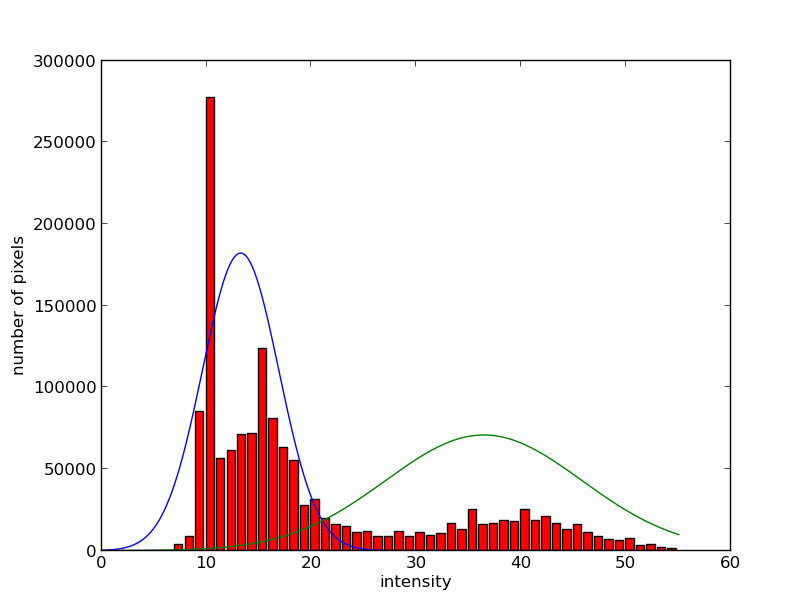
\includegraphics[scale=0.4]{Figures/segmentation/temp_hist_prez}
	\end{center}
	\label{img:Approx}
	\caption{An EM approximation of an image histogram}
\end{figure}

\begin{figure}
	\begin{center}
		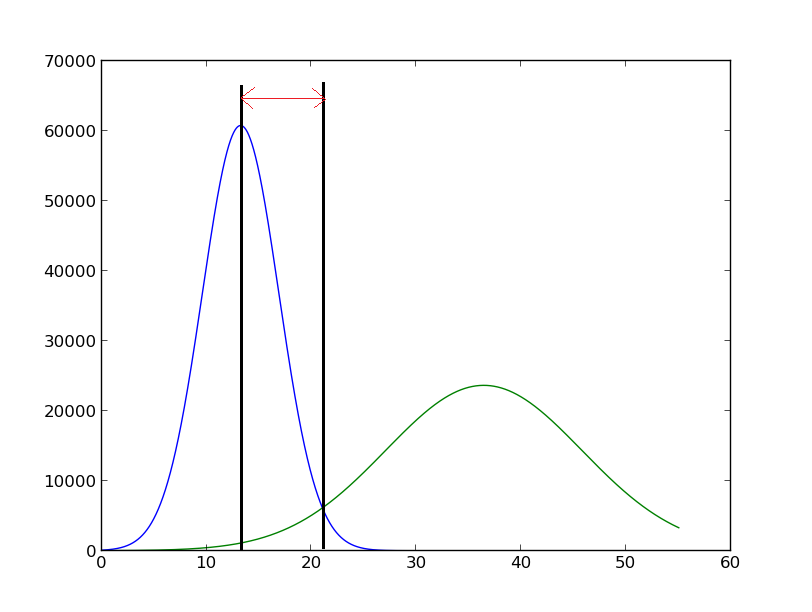
\includegraphics[scale=0.4]{Figures/segmentation/approx_hist_thr}
	\end{center}
	\label{img:Thr}
	\caption{A calculation of a threshold}
\end{figure}

The point of using the background segmentation step is to overcome a problem of undetected cells that expose a low intensity. To evaluate this step, the optimal threshold for each image in the dataset was determined manually. The evaluation was performed in two ways - on object and pixel level. First, in the object level evaluation, the number of detected cells was compared to the ground truth, as the number of cells in each image is known in advance. Second, segmented regions were compared to the ground truth. As a measure of similarity \textit{precision} and \textit{recall} are used . This measure should indicate a similarity of obtained segmentation to a manually segmented cells. \\

Table \ref{tab:Object} summarizes the object level results. The results show that the Region growing approach usually detects more objects than contained in the ground truth segmentation. Those extra objects detected by the proposed approach are actually partial cells that were removed from the ground truth segmentation. The presence of those partial cells demonstrates the advantages and sensitivity of region growing, but also raises a question should those cells be eliminated from further process or used as a \textit{fully observed} cells.

Table \ref{tab:Pix} summarizes the pixel level results. The proposed approach is compared with the two approaches by Huang et al. mentioned in \ref{Chapter3}. Precision and recall are expressed by true positives (TP), false positive (FP) and false negative (FN). True positive are the pixels that are contained both in the ground truth and the segmentation achieved by the proposed method. False positives are the pixels that does not belong to the ground truth but are present in the achieved segmentation, while false negatives are the pixels that belong to the ground truth but are not present in the achieved segmentation. Precision is then defines as $\frac{TP}{TP + FP}$ while recall equals $\frac{TP}{TP + FN}$. Informally, precision can be seen as a confidence that the segmented region belongs to the cell, while recall can be seen as a proportion of a cell the segmentation has found. It can be seen that the previous approaches usually have high precision but low recall. With the proposed approach, those measures are much more balanced which suggests that the obtained contours represent follow the cells outline much better.

\begin{table}
	\begin{center}

	\caption{Number of detected and overlapping cells}
	\label{tab:Object}
	\begin{tabular}{|p{2cm}|p{2cm}|p{2cm}|p{2cm}|}
	\textbf{image ID} & objects & detected objects & overlapping objects \\
	\hline 
	\hline 
	01 & 64 & 69 & 35 \\
	02 & 52 & 63 & 13 \\
	03 & 93 & 99 & 38 \\
	04 & 73 & 73 & 28 \\
	05 & 52 & 52 & 16 \\
	06 & 77 & 77 & 36 \\
	07 & 62 & 62 & 28 \\
	08 & 60 & 60 & 27 \\
	09 & 52 & 55 & 16 \\
	10 & 36 & 42 & 13 \\
	11 & 49 & 56 & 16 \\
	12 & 57 & 60 & 49 \\
	13 & 52 & 57 & 25 \\
	14 & 67 & 78 & 33 \\
	15 & 68 & 76 & 58 \\
	16 & 44 & 48 & 16 \\
	17 & 20 & 20 & 6 \\
	18 & 43 & 53 & 15 \\
	19 & 70 & 77 & 4 \\
	20 & 49 & 49 & 11 \\
	21 & 66 & 70 & 9 \\
	22 & 120 & 127 & 76 \\
	23 & 53 & 56 & 15 \\
	24 & 75 & 85 & 45 \\
	25 & 24 & 24 & 14 \\
	26 & 47 & 47 & 47 \\
	27 & 44 & 44 & 40 \\
	28 & 13 & 13 & 6 \\
	\hline
	\end{tabular}
	\end{center}
\end{table}

\begin{table}
	\caption{Pixel level results for each pattern}
	\label{tab:Pix}
	\begin{tabular}{|c||c|c||c|c||c|c|}
	\hline
	 & \multicolumn{2}{c}{Proposed method} & \multicolumn{2}{c}{MULTISTAGE} & \multicolumn{2}{c}{AutoLearning} \\
	\hline
	 \textbf{Pattern} & Prec & Rec & Prec & Rec & Prec & Rec \\
	 \hline
	 \hline
	 homogeneous & 0.836 & 0.96 & 0.955 & 0.58 & 0.983 & 0.467 \\
	 centromere & 0.7986 & 0.84 & 0.628 & 0.395 & 0.846 & 0.356 \\
	 nucleolar & 0.825 & 0.743 & 0.667 & 0.389 & 0.828 & 0.44 \\
	 cytoplasmatic & 0.706 & 0.8293 & 0.166 & 0.374 & 0.553 & 0.269 \\
	 coarse speckled & 0.721 & 0.9 & 0.664 & 0.55 & 0.928 & 54.2 \\
	 fine speckled & 0.748 & 0.94 & 0.81 & 0.499 & 0.941 & 0.547 \\
	 \hline
	\end{tabular}
\end{table}


%------------------------------------------------------%
%                                                      %
%               PRIOR POSITIONING                      %
%                                                      %
%------------------------------------------------------%

\section{Positioning of a prior shape}

Once the background has been found, a rough estimate of cell positions in known. Still, a lot of cells overlap. In order to split them, we will make use of the circularity properties of cells. If circles of cells could be detected, or at least circular parts of cells, they might be split. To detect circles the Hough transformation is used.

\subsection{Hough transformation for circles}

The Hough transformation is a general voting procedure used in Computer vision. The outline of the method is given in algorithm \ref{alg:Hough}. It discretizes a parameter space and assigns every bin a number of votes proportional to the number of edges in an image that could be generated with those specific bin parameters. In this case, each bin represents one candidate circle in an image with the equation 

\begin{equation}
	\mathcal{H}(\hat{x}, \hat{y}, r) = (\hat{x} - x)^2 + (\hat{y} - y)^2 = r^2,
\end{equation}

where  $\hat{x}$ and $\hat{y}$ represent the origin of a circle and $r$ its radius. Now every edge point in an image \textit{votes} for every bin that could have generated it, under the assumption that the edge is a part of a circle. \\

\begin{algorithm}
	\caption{Hough Transform}
 	\label{alg:Hough}
 	\begin{algorithmic}[1]
 	\Function{Hough Transformation}{}
 		\State initialize accumulator $\mathcal{H}$ to all zeros
 		\For{ each edge in image }
 			\State increment every cell $\mathcal{H}(x,y,r)$ which could be the center of a circle
 		\EndFor
 		\State search for local maxima cells of $\mathcal{H}$
 	\EndFunction
\end{algorithmic}
\end{algorithm}

After voting, every local maximum is selected as a circle. Additionally, every vote could be weighted proportionally to its magnitude. Note that not all local maxima are actual circles. Although quite straightforward, the method can easily become unfeasible. Searching for all radius' is obviously unfeasible for large images, so any restriction on circle size range is most certainly helpful. To help the search, the radius is limited to range from the smallest to the largest radius found in the data set. \\

Another problem with the Hough transformation is its sensitivity to noise. If we assume there is an uniform noise in an image, it is easy to conclude that it might imply false circles over an image. Methods to overcome that problem usually include better discretization of parameters or smoothing in the accumulator by incrementing neighboring bins, but for a fully automated application this is not a suitable solution. Instead, information about the background extracted in the previous step could be used. As we can obtain the background quite successfully, every circle with a center in the background region can be removed, like every other circle which has similar properties as the background circles. As a criteria here, a mean intensity in the green channel is used - every circle with a mean intensity lower than the highest mean intensity found in the background is removed. Figure \ref{fig:Hough} illustrates that selection. Now each circle serves as a seed point for precise segmentation of contours and splitting overlapping cells.

\begin{figure}
	\begin{minipage}[h]{0.49\linewidth}
		\begin{center}
			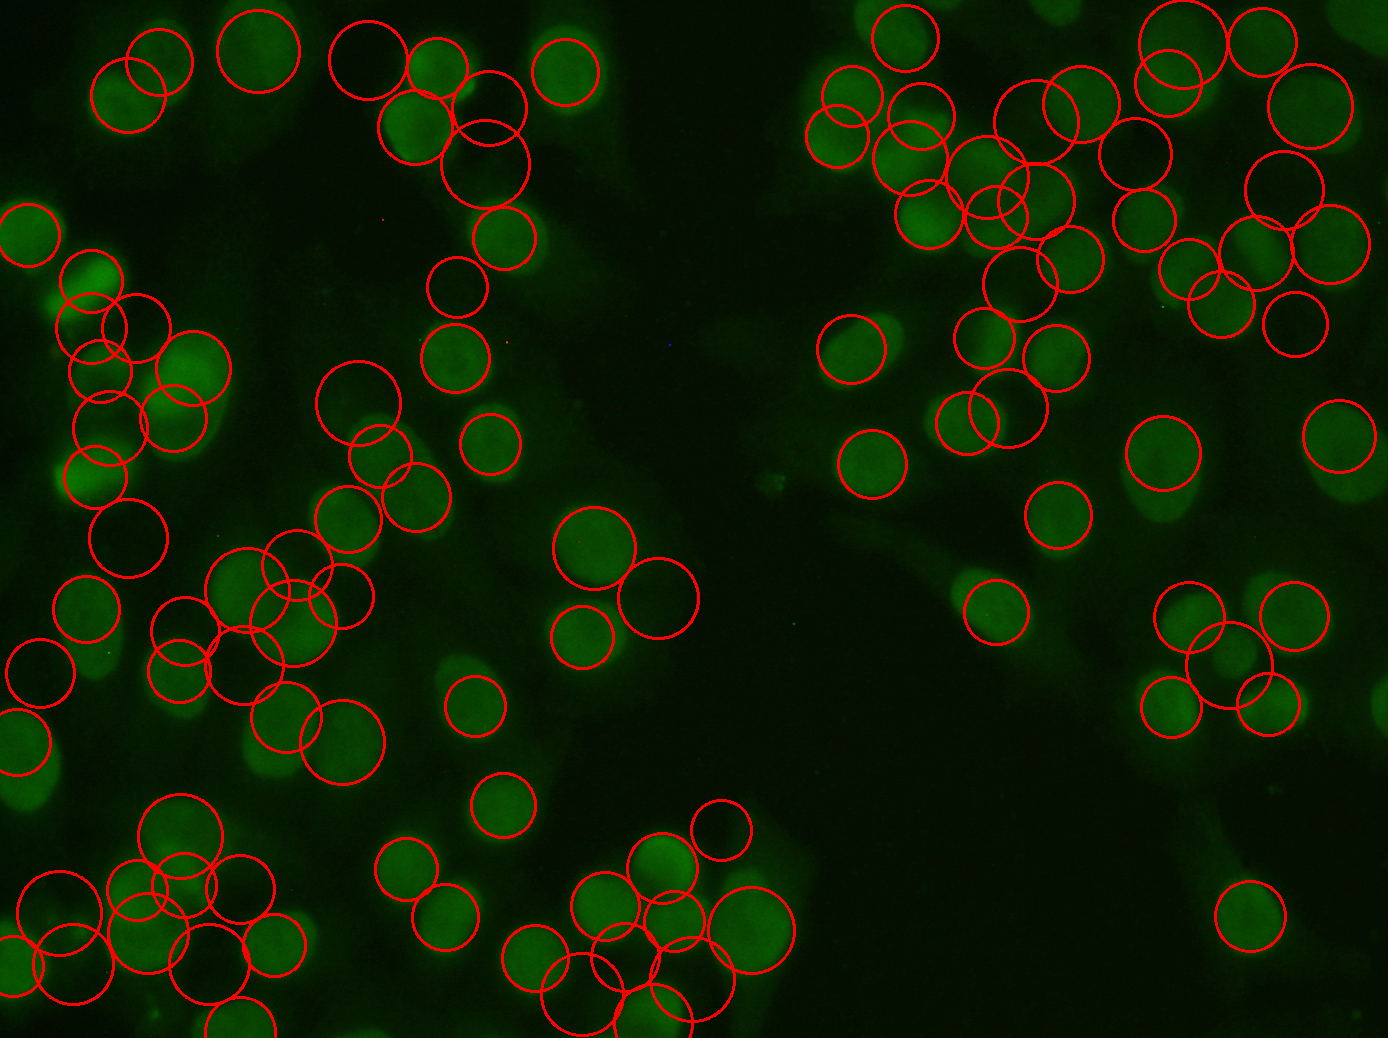
\includegraphics[scale=0.13]{Figures/segmentation/circles_no_selection}
			\\ (a)
		\end{center}	
	\end{minipage}
	\begin{minipage}[h]{0.49\linewidth}
		\begin{center}
			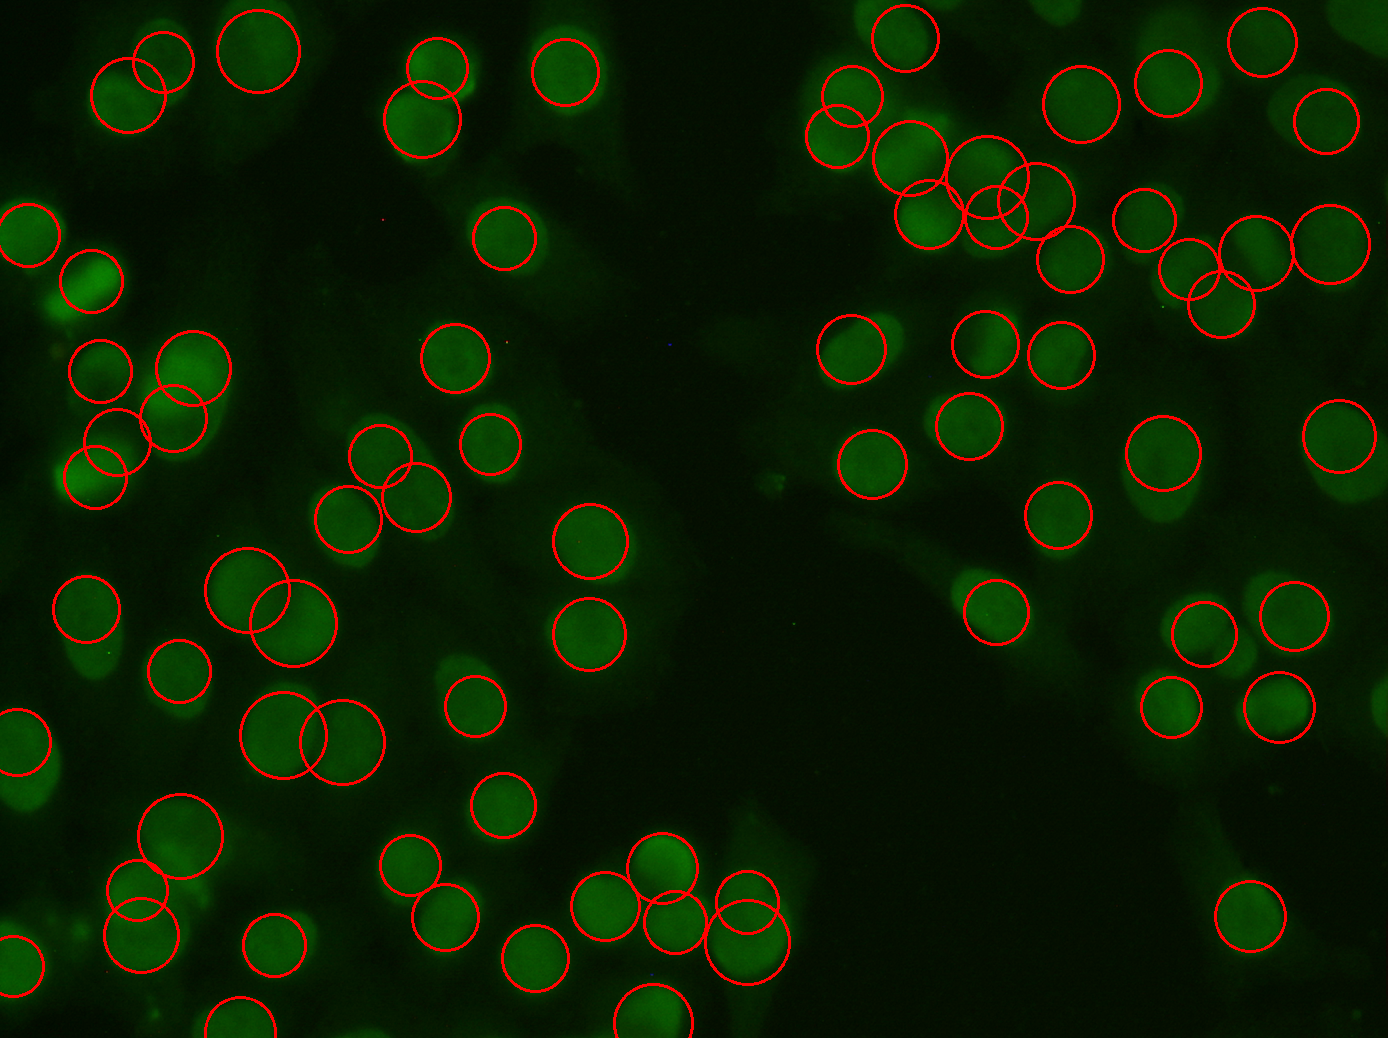
\includegraphics[scale=0.13]{Figures/segmentation/circles_after_selection}
			\\ (b)
		\end{center}
	\end{minipage}
	\caption{Hough transformation with all detected circles (a) and after removing background circles (b)}
	\label{fig:Hough}
\end{figure}

%-----------------------------------------------------%
%                                                     %
%             SEGMENTATION                            %
%                                                     %
%-----------------------------------------------------%

\section{Precise contours with Morphological snakes}

Morphological snakes or active contour methods are one very popular computer vision method. This method employs an energy optimization approach where it tries to minimize the energy function induced by a curve.  The minimum is usually found by a steepest descent approach. \\

As the images can be quite noisy, a specific version of morphological snakes called \textit{Active contour without edges} (ACWE) is used. The ACWE doesn't need well defined borders and it is less sensitive to the initial configuration and model parameters. Due to the noisy nature of images used in this process, the ACWE has the potential to successfully deal with the noise. The Active contour methods try to adjust the starting contour to a local minimum by iteratively solving a time-dependent partial differential equations (PDE). However, solving the PDE is computationally costly and often has stability issues. \\

The most efficient approaches avoid to solve the PDE directly. The key idea that allows the simplification of the problem is that the curve is implicitly  represented by the set of image points neighboring the target area. The evolution of the curve is then achieved by elimination and introduction of points in the target set. Any geometric property can be approximated with local operations on the set of points. Those methods are based on mathematical morphology and make use of morphological operators such as \textit{erosion} and \textit{dilation} to approximate the PDEs. For the equivalence of differentiation and morphological operators see \cite{Pami2013}.




\subsection{Background }

This section summarizes the most important parts of curve evolution with PDEs and morphological operators.




\subsubsection{Contour evolution with PDEs}

Differential operators are key to contour evolution with PDEs -- the change of contour is given by a differential operator. \\

Let $\mathcal{C}$ be a parametrized 2D curve over time so that $\mathcal{C}: \mathbb{R}^+ \times [0,1] \rightarrow \mathbb{R}^2 : (t,p) \rightarrow \mathcal{C}(t,p)$. A differential operator $\mathcal{L}$ defines the curve evolution with PDE $\mathcal{C}_t = \mathcal{L}(\mathcal{C})$. The result of evolution depends on the differential operator. There are many forms in which it can be written but one popular is $\mathcal{L} = \mathcal{F} \cdot \mathcal{N}$, where $\mathcal{N}$ is the normal to the curve and $\mathcal{F}$ is a scalar field which determines the speed of evolution. \\

A particularly interesting form is the one in which $\mathcal{L}$ is defined with $\mathcal{F} \in \{ -1,1 \}$. Such an operator evolves the curve along its normal direction with constant speed. If $\mathcal{F}$ takes the form of the Euclidean curvature of $\mathcal{C}$, then the problem is convex so it will converge to the optimal solution. \\

With the explicit representation of the curve certain problems occur. It is not easy to deal with topological changes and re-parameterization of the curve. An alternative to the explicit representation is an implicit one. Let $u: \mathbb{R}^+ \times \mathbb{R}^2 \rightarrow \mathbb{R}$ an implicit representation of $\mathcal{C}$ such that $\mathcal{C}(t) = \{ (x,y); u(t,(x,y)) = 0 \}$. When $\mathcal{C}_t = \mathcal{F} \cdot \mathcal{N}$, the curvature evolution of any function $u(x,y)$ which embeds the curve is $\frac{\partial u}{\partial t} = \mathcal{F}|\nabla u|$. \\

With that in mind, the PDEs that are of interest to the curvature evolution are

\begin{equation}
	\frac{\partial u}{\partial t} = \pm |\nabla u|
	\label{eq:PDE1}
\end{equation}

\begin{equation}
	\frac{\partial u}{\partial t} = div \left ( \frac{\nabla u}{|\nabla u|}  \right ) \cdot |\nabla u|
	\label{eq:PDE2}
\end{equation}

where $\mathcal{F} = \pm 1$ in \ref{eq:PDE1} and $\mathcal{F} = \mathcal{K}$ for \ref{eq:PDE2}. $\mathcal{K}$ denotes the Euclidean curvature.



\subsubsection{Morphological operators} 

Morphological operators are monotone operators that are translation- and contrast- invariant. Every morphological operator $T$ can be represented in a $sup-inf$ representation of form 

\begin{equation}
	(T_hu)(\mathbf{x}) = \sup_{B \in \mathcal{B}} \inf_{\mathbf{y} \in \mathbf{x} + hB}u(\mathbf{y})
\end{equation}

or a dual $inf-sup$ form

\begin{equation}
	(T_hu)(\mathbf{x}) = \inf_{B \in \mathcal{B}} \sup_{\mathbf{y} \in \mathbf{x} + hB}u(\mathbf{y}),
\end{equation}

where $\mathcal{B}$ is a set of structuring elements that uniquely defines the operator and $h$ is the size of operator. \\

The most common morphological operators are dilation and erosion. A dilation $D_h$ with radius $h$ of function $u$ is defined as 

\begin{equation}
	D_hu(\mathbf{x}) = \sup_{\mathbf{x} \in hB(0,1)} u(\mathbf{x} + \mathbf{y})
\end{equation}

while the erosion has a similar form

\begin{equation}
	E_hu(\mathbf{x}) = \inf_{\mathbf{x} \in hB(0,1)} u(\mathbf{x} + \mathbf{y}),
\end{equation}

 where $B(0,1)$ is a ball of radius 1 centered at 0 and $h$ is the scaling factor.
 
\subsubsection{Curvature operator}

A curvature operator works as follows. Let $SI_h$ and $IS_h$ be respectively $sup-inf$ and $inf-sup$ morphological operators with a base $\mathcal{B}^2 = \{ [-1,1]_{\theta} \subset \mathbb{R}^2 : \theta \in [0, \pi) \}$. The base is made of all segments of length 2 centered at the origin. It can be proven that the successive application of \textit{a mean operator}, for a very small $h$, is equivalent to the curvature flow of PDE \ref{eq:PDE2}. \\

The mean operator is now defined as a composition of two morphological operators

\begin{equation}
	T_{h/2}^2 \ocircle T_{h/2}^1 \approx \frac{T_h^2u + T_h^1u}{2}.
\end{equation}

\subsection{Morphological snakes}

It can be proven that the above mentioned morphological operators - dilation, erosion and the curvature flow operator - behave infinitesimally like PDEs \ref{eq:PDE1} and \ref{eq:PDE2}. In that context, given the curvature evolution function which includes both terms \ref{eq:PDE1} and \ref{eq:PDE2}, those operators may be used to evolve the contour by approximating the solution to the PDEs. \\

The ACWE uses an energy function for image segmentation which takes into account the content of the interior and exterior regions of the curve. The function of a curve $\mathcal{C}$ used in the ACWE looks like

\begin{equation}
	\begin{split}
		F(c_1,c_2, \mathcal{C}) & = \mu \cdot \mathtt{length}(\mathcal{C}) + \upsilon \cdot \mathtt{area}(\mathtt{inside}(\mathcal{C})) \\
	 & + \lambda_1 \int_{\mathtt{inside}(\mathcal{C})} \Vert I(\mathbf{x}) - c_1 \Vert d\mathbf{x} +   \lambda_2 \int_{\mathtt{outside}(\mathcal{C})} \Vert I(\mathbf{x}) - c_2 \Vert d\mathbf{x}
	\end{split}
	\label{eq:Functional}
\end{equation}

where $I$ represent the image and the non-negative parameters $\mu, \upsilon, \lambda_1, \lambda_2$ controls the strength of factors. The solution is now found as 

\begin{equation}
	\min_{c_1,c_2, \mathcal{C}} F(c_1,c_2, \mathcal{C}),
\end{equation}

which is a bit challenging problem. The problem could be relaxed by calculating the parameters given a fixed contour. The values $c_1$ and $c_2$ that minimize $F$ are given as the mean of the values of $I$ inside and outside of the contour
	
\begin{equation}
	c_1(\mathcal{C}) = \frac{\int_{\mathtt{inside}(\mathcal{C})}I(\mathbf{x})d\mathbf{x}}{\int_{\mathtt{inside}(\mathcal{C})}d\mathbf{x}}
\end{equation}

\begin{equation}
	c_2(\mathcal{C}) = \frac{\int_{\mathtt{outside}(\mathcal{C})}I(\mathbf{x})d\mathbf{x}}{\int_{\mathtt{outside}(\mathcal{C})}d\mathbf{x}}.
\end{equation}

The evolution of the contour is now given with the Euler-Lagrange equation of functional \ref{eq:Functional}

\begin{equation}
	\begin{split}
		\frac{\partial u}{\partial t} & = | \nabla u | \left ( \mu \cdot \mathtt{div} \left ( \frac{\nabla u}{|\nabla u|}  \right ) - \upsilon - \lambda_1(I - c_1) -\lambda_2 (I - c_2) \right ) .
	\end{split}
\end{equation}

This equation specifies the direction the contour should evolve to minimize the functional $F$ in the steepest descent manner. The factor 

\begin{equation}
	|\nabla u| \cdot \upsilon
\end{equation} 

is called the \textit{balloon force} and it determines the strength of fragments in the contour : when this term is strong the fragment of the contour is far from the target region and it reduces as the fragment approaches the target region. This factor is approximated with the dilation and erosion operators and it represents the approximation of the PDE \ref{eq:PDE1}. \\

The factor

\begin{equation}
	| \nabla u | \cdot \mu \cdot \mathtt{div} \left ( \frac{\nabla u}{|\nabla u|}  \right )
\end{equation}

is called the \textit{smoothing force} which represent a weighted version of the mean curvature divergence and corresponds to the PDE \ref{eq:PDE2}. The $\mu$ controls the strength of the smoothing operator at each point. This factor is approximated with the mean curvature operator. \\

The remainder of the equation determines should a point be included in or excluded from the current region, or stay where it is. If $\lambda_1(I - c_1) < \lambda_2 (I - c_2) $ at $\mathbf{x}$, then $\mathbf{x}$ should be included in the current region, or excluded if the inequality is reversed. If $\lambda_1(I - c_1) = \lambda_2 (I - c_2) $ $\mathbf{x}$ should stay where it is. \\

Finally, the ACWE algorithm is given with these three successive steps

\begin{equation}
	u^{n + \frac{1}{3}}(\mathbf{x}) = 
	\begin{cases}
		(D_hu^n)(\mathbf{x}) & \text{if } \upsilon < 0 \\
		(E_hu^n)(\mathbf{x}) & \text{if } \upsilon > 0 \\
		u^n(\mathbf{x}) & \text{otherwise}
	\end{cases}
\end{equation}

\begin{equation}
	u^{n + \frac{2}{3}}(\mathbf{x}) = 
	\begin{cases}
		1 &\text{if } |\nabla u^{n + \frac{1}{3}}|(\lambda_1(I - c_1)^2 < \lambda_2 (I - c_2)^2)(\mathbf{x}) < 0 \\
		0 &\text{if } |\nabla u^{n + \frac{1}{3}}|(\lambda_1(I - c_1)^2 < \lambda_2 (I - c_2)^2)(\mathbf{x}) > 0 \\
		u^{n + \frac{1}{3}} & \text{otherwise}
	\end{cases}
\end{equation}

\begin{equation}
	u^{n + 1}(\mathbf{x}) = \left ( (SI_h \ocircle IS_h)^{\mu} u ^{n + \frac{2}{3}}  \right )(\mathbf{x}).
\end{equation}

The only question that remains to be answered is how to set the initial curve. As the initial curves, the circles detected in the previous step are used. \\

Table \ref{tab:Snakes} summarizes the results obtained with the morphological snakes. This method reduced the number of overlapping cells significantly. Still, a problem occurs with the \textit{nucleolar} and \textit{centromere} patterns which have bright organelles. These patterns are usually oversegmented -- the output of the segmentation are organelles, not the whole cell (Figure \ref{img:oversegmentedSnakes}). Although those organelles help to split the overlapping cells, they are not the target objects. How to effectively  overcome this problem is a problem for future research, but for now, a \textit{convex envelope} of segmentation results was used. \\ 

\begin{table}
	\centering
	\begin{center}

	\caption{Number of overlapping cells after snakes}
	\label{tab:Snakes}
	\begin{tabular}{|p{2cm}|p{2cm}|p{2cm}|p{2cm}|}
	\textbf{image ID} & cells &  overlapping - before &  overlapping - after \\
	\hline 
	\hline 
	01 & 64 & 35 & 16 \\
	02 & 52 & 13 & 2 \\
	03 & 93 & 38 & 5 \\
	04 & 73 & 28 & 7 \\
	05 & 52 & 16 & 2 \\
	06 & 77 & 36 & 10 \\
	07 & 62 & 28 & 6 \\
	08 & 60 & 27 & 5 \\
	09 & 55 & 16 & 10 \\
	10 & 42 & 13 & 5 \\
	11 & 49 & 16 & 6 \\
	12 & 60 & 49 & 8 \\
	13 & 52 & 25 & 6 \\
	14 & 67 & 33 & 6 \\ 
	15 & 68 & 58 & 40 \\
	16 & 44 & 16 & 5 \\
	17 & 20 & 6 & 2 \\
	18 & 43 & 15 & 4 \\
	19 & 70 & 4 & 0 \\
	20 & 49 & 11 & 6 \\
	21 & 66 & 9 & 2 \\
	22 & 120 & 76 & 27 \\
	23 & 53 & 15 & 5 \\
	24 & 75 & 45 & 20 \\
	25 & 24 & 14 & 6 \\
	26 & 47 & 47 & 23 \\
	27 & 44 & 40 & 24 \\
	28 & 13 & 13 & 2 \\
	\hline
	\end{tabular}
	\end{center}
\end{table}

\begin{figure}
	\begin{minipage}[h]{0.49\linewidth}
		\begin{flushright}
			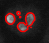
\includegraphics[height=2cm]{Figures/segmentation/oversegmented_nucleolar}
		\end{flushright}
	\end{minipage}
	\hspace{0.3cm}
	\begin{minipage}[h]{0.49\linewidth}
		\begin{flushleft}
			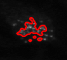
\includegraphics[height=2cm]{Figures/segmentation/oversegmented_centromere}
		\end{flushleft}
	\end{minipage}
	\caption{Oversegmented results}
	\label{img:oversegmentedSnakes}
\end{figure}

\begin{table}
	\begin{center}
	\caption{Pixel level results for each pattern, with and without convex envelope}
	\label{tab:SnakesPix}
	\begin{tabular}{|c||c|c||c|c|}
	\hline
	 & \multicolumn{2}{c}{Snakes without envelope} & \multicolumn{2}{c}{Snakes with envelope}  \\
	\hline
	 \textbf{Pattern} & Prec & Rec & Prec & Rec\\
	 \hline
	 \hline
	 homogeneous & 0.961 & 0.975 &  0.962 & 0.978  \\
	 centromere & 0.87 & 0.54 & 0.92 & 0.74  \\
	 nucleolar & 0.96 & 0.48 & 0.97 & 0.76  \\
	 cytoplasmatic & 0.826 & 0.54 & 0.786 & 0.61 \\
	 coarse speckled & 0.941 & 0.977 & 0.948 & 0.974 \\
	 fine speckled & 0.956 & 0.94 & 0.932 & 0.94 \\
	 \hline
	\end{tabular}
	\end{center}
\end{table}

Table \ref{tab:SnakesPix} summarizes the segmentation performance with the morphological snakes, with and without the convex envelope. The results suggest that the \textit{ compact} patterns like homogeneous and speckled patterns have been segmented very successfully with the morphological snakes. On the other side, patterns like centromere and nucleolar, so as cytoplasmatic encounter certain problems in images with positive fluorescence intensity. Those problems are caused by bright organelles, or rim in a cell's body. As such organelles are very bright, they attracted the contour much more than an uniform body of a cell. Those differences are much less expressed in a low intensity images. The usage of the convex envelope of a segmented region improves the segmentation results and does not effect the segmentation of the other patterns significantly.  